\chapter{Region Based Convolutional Neural Network}
\section{The Problem Of Region Of Interest}
\label{section:problemofROI}
\noindent
	Computer vision is a large field that has been attracted lots of researchers, scientists in the recent years (after AlexNet’s milestone). Beside image classification problem, another research trend of computer vision is object detection. The difference between two types of problem is that classification problem wants to know the label or labels of the image, while detection problem try to locate a bounding box surrounding the object inside the image. The challenge is there could be many bounding boxes representing different objects and we do not how many beforehand. The major reason why typical CNN models as we describe in section 2 cannot solve this problem is that the length of the output layer is not constant (unknown number of objects). A naive approach for this is that we can take different region of interest (RoI) and apply CNN model to check whether the RoI has object. Yet, this approach also has a huge problem is that the RoIs may have different spatial locations in the image, therefore, it will cost an expensive computational resource because of a huge number of RoIs.
	
\section{The Original R-CNN}
\label{section:rcnn}
\noindent

	In 2014, a new model had been proposed named region based convolutional neural network. The model has a remarkable record on PASCAL VOC 2010 with the mean average precision (mAP) of 53.7\% and mAP of 31.4\% on ILSVR2013 detection dataset \cite{rcnn}.
	
	To solve the issue of the numerous Rois, Ross Girshick et al. proposed a method where we use selective search to extract just 2000 regions from the image and he called them region proposals \cite{rcnn}. As a result, instead of blowing up the computational resource to classify RoIs like the naive approach, now we can just work with 2000 regions.
	
	According to the author, their system consists of three modules. The first module is the one that solve the expensive computation issue by using selective search to generate category-independent region proposals. The second module is a CNN that extract a 4096-dimensions feature vector from RoIs as the output. The last one is a set of SVMs and a linear regression models to classify the object and predict its bounding box, respectively.
	
	%Figure RCNN
	
	Problems with R-CNN:
	\begin{itemize}
		\item Training is a multi-stage pipeline and expensive in space and time.
		\item It cannot be implemented as real time system because it takes 47s/image to extract features from RoIs when using VGG16 as backbone (on a GPU).
		\item The selective search algorithm is a fixed algorithm. Therefore, no learning is happening at that stage. This could lead to the generation of bad candidate region proposals.
	\end{itemize}

\section{The Improvement In Fast R-CNN And Faster R-CNN}
\label{section:fastandfasterrcnn}
\noindent
	
	Next year, in 2015, Ross Girshick et al again proposed a new model called Fast R-CNN which solved the drawbacks of their previous model. This model architecture looks similar to the original R-CNN but instead of feeding the RoIs to CNN, an input image and multiple regions of interest (RoIs) are input into a CNN. Each RoI is pooled into a fixed-size feature map and then mapped to a feature vector by fully connected layers (FCs). The network has two output vectors per RoI: softmax probabilitiesand per-class bounding-box regression offsets. The architecture is trained end-to-end with a multi-task loss \cite{fastrcnn}.
	
	Fast R-CNN has several advantages according to the paper:
	\begin{itemize}
		\item Higher detection quality (mAP) than R-CNN.
		\item Training is single-stage, using a multi-task loss.
		\item Training can update all network layers.
		\item No disk storage is required for feature caching.
	\end{itemize}
	
	With Fast R-CNN, we do not have to feed 2000 RoIs to CNN which enhance the training and testing speed by execute the convolution once per image and feature map will be generated from it. The network is illustrated in figure 6 (below).
	
	Both of the above models (R-CNN \& Fast R-CNN) use selective search to generate the RoIs. However, selective search is a slow and time-consuming process affecting the performance of the network \cite{fasterrcnn}. Therefore, Shaoqing Ren et al came up with an object detection algorithm that alternates the selective search algorithm and allows the network completely learn to propose the RoIs and they called it Region Proposal Networks (RPNs). By sharing convolutional layers, the marginal cost for computing proposals is significantly decrease (e.g., 10s/image) \cite{fasterrcnn}.
	
	As an upgrade from Fast R-CNN, the new model was introduced in 2016 by Shaoqing Ren et al called Faster R-CNN that improves the speed of the model towards real-time object detection. This new architecture is similar to its predecessor that image is provided as an input to a convolutional network to generate feature maps. Yet, instead of applying selective search, a separated network called RPNs (which is completely trained) is used to predict RoIs. In the next stage, the predicted results are reshaped using a RoIs pooling layer. And then, the rectangular RoIs are used for classifying the objects inside the image and predicting the offset value of bounding boxes.
	
	%table 1
	\begin{table}
		\begin{tabularx}{1\textwidth} {
				| >{\raggedright\arraybackslash}X 
				| >{\raggedright\arraybackslash}X
				| >{\raggedright\arraybackslash}X 
				| >{\raggedright\arraybackslash}X  
				| >{\raggedright\arraybackslash}X | }
			\hline
			Model & Describe & Testing speed & Limitations \\
			\hline
			CNN & Divides the image into multiple regions and then classify each region into various classes.  & unknown & Naive approach take a huge number of regions to predict, therefore, expensive computation cost. \\
			\hline
			R-CNN & Apply selective search, choose 2000 regions to process separately.  & 47s on VOC07 & Expensive computation cost from difference CNN models for each region \\
			\hline
			Fast R-CNN & Extract feature maps first then apply selective search to generate regions.  & 0.32s on VOC07 & Selective search is slow and un-trainable. \\
			\hline
			Faster R-CNN & Alternate selective search by RPN which can be trainable and much faster.  & 0.2s on both COCO and VOC07 & Object proposal takes time and as there are different systems working one after the other, the performance of systems depends on how the previous system has performed. \\
			\hline
		\end{tabularx}
		\caption{Comparison between CNN, R-CNN, Fast R-CNN, and Faster R-CNN}
		\label{table:comparisonofrcnns}
	
	\end{table}
%	\begin{table}[!htp]
%		\centering
%		\begin{tabular}{|m{5cm}|m{1cm}|m{1cm}|m{1cm}|} 
%			\hline
%			a4 & b4 & c4 & d4 & \hline
%			a4 & b4 & c4 & d4 & \hline
%			a4 & b4 & c4 & d4 & \hline
%			a4 & b4 & c4 & d4 & \hline
%		\end{tabular}
%		
%	\end{table}
	
	
\section{Region Proposal Network (RPNs)}
\label{section:rpns}
\noindent	

	In object detection using region based technique, RPN is a one true backbone which takes an image as the input and outs a set of rectangular RoIs. Although the RPN can process a whole image, the ultimate goal of the author is to share computation with the Fast R-CNN. As the result, the RPN is modified to be a small network that works as the second stage in the model architecture and it take the convolutional feature map output by the last shared convolutional layer of Faster R-CNN object detection network as the input. And then, this small network slide a n x n spatial window over the feature map to map it from high dimensional feature to lower one. This feature then is fed to two siblings fully-connected layers - a box-regression layer and a box-classification layer \cite{fasterrcnn}.
	
	\begin{figure}[H]
		\centering
		{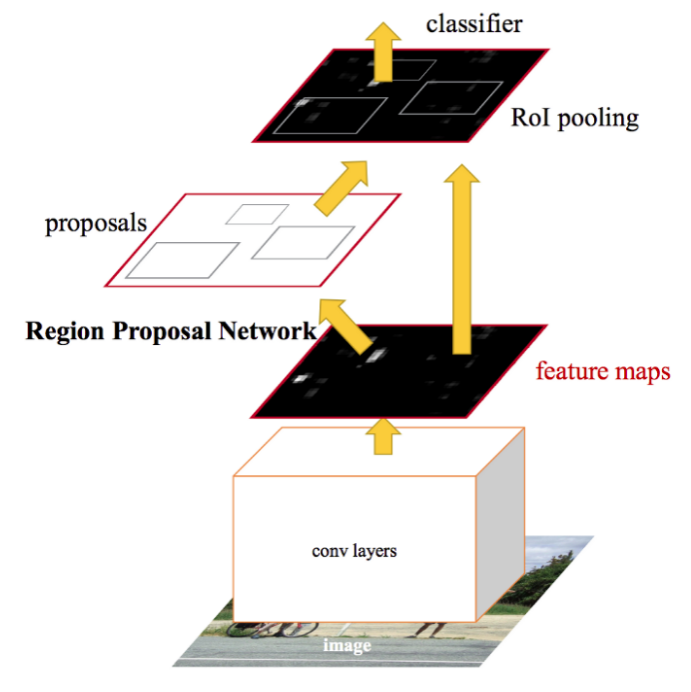
\includegraphics[width=0.7\textwidth]{./hinhanh/chap4/faster_rcnn.png}}
		\caption{Faster R-CNN architect including RPN.}
	\end{figure}
	
\subsection{Anchors}
\label{subsection:anchors}
\noindent		

	At each sliding window position, we predict simultaneously lots of proposals with k is denoted as the maximum number of proposals at each location. According to the paper, the regression layer has 4k predicted coordinates of k boxes and classification layer has 2k predicted probability outputs of object or not object for each proposals. Therefore, the k value helps the authors parameterize the unknown number of boxes to k boxes and they called them anchors. 
	An anchor is defined as the centered boxes of each sliding window. Based on the paper, the authors used 1 square, 2 rectangles with 3 scales and 3 aspect ratio to create 9 anchors (so k = 3 x 3 = 9). Therefore, with a feature map of the size W x H there are WHk anchors in total. These anchors are labeled with positive or negative based on the area that overlap with the ground truth box as the following rule:
	\begin{itemize}
		\item The anchor is positive when it is the maximum value of intersection over union (IoU) and it is bigger than 0.7.
		\item The anchor is negative when it is smaller than 0.3.
		\item The anchor that neither positive nor negative does not consider to be the training objective.
	\end{itemize}
	
\subsection{ROI Pool Layer}
\label{subsection:roi_pool}
\noindent	
	
	For each object proposal, RoI pooling layer extracts a fixed length of feature vector from the feature map so that it can be fed into the classifier and regressor in the final FC layer. More explicitly, the RoI pooling can be described in three steps:
	\begin{itemize}
		\item Dividing the region proposal into equal-sized sections (the number of which is the same as the dimension of the output).
		\item Finding the largest value in each section.
		\item Mapping these max values to the output buffer.
	\end{itemize}
	
	\begin{figure}[H]
		\centering
		{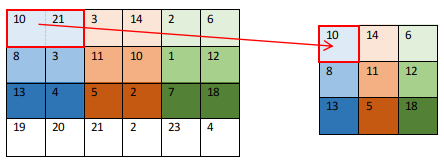
\includegraphics[width=0.8\textwidth]{./hinhanh/chap4/roi_quantization.png}}
		\caption{An example of RoI pooling window size 3x3 on vector 4x6.}
		\label{fig:roi_quantization}
	\end{figure}
	
	As we can see on \ref{fig:roi_quantization}, RoI pooling only take 1x2 vector to map its maximum value to a fixed length vector because quantization process (4/3 $\sim$ 1.3333 = 1, 6/3 = 2). Therefore, the entire bottom row does not take in to account causing missing information of the feature map. This process will directly affect the result accuracy.
	
	
	
	
	
	
	
	
	
	
	
	
	